\documentclass{article}
\usepackage[utf8]{inputenc}
\usepackage{amsmath,amssymb,amsthm,mathrsfs,graphicx}
\usepackage{float}

\title{HW8}
\author{Ry Wiese\\wiese176@umn.edu}
\date{December 2, 2019}

\begin{document}

\maketitle

All results can be reproduced by running HW8.m. I commented out the lines that generate plots.

\section{Problem 1}

\subsection{Part i}

Using the gradient descent method with golden section search gave me an optimal solution of $\mathbf{x} = \left( \begin{array}{cc} -2.1418\\2.8582 \end{array} \right)$ and an optimal value of -4.1423.

\begin{figure}[H] % "h" is where to place, h=here, t=top, b=bottom
  \centering
  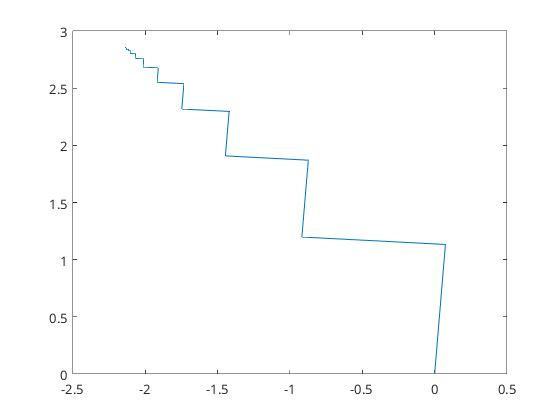
\includegraphics[angle=0,totalheight=50mm]{P1igraph.jpg}
  \caption{Gradient Descent with Golden Search Solution Path}
  \label{fig:tabl}
\end{figure}

\subsection{Part ii}

Using the gradient descent method with backtracking line search gave me an optimal solution of $\mathbf{x} = \left( \begin{array}{cc} -2.1418\\2.8582 \end{array} \right)$ and an optimal value of -4.1423.

\begin{figure}[H] % "h" is where to place, h=here, t=top, b=bottom
  \centering
  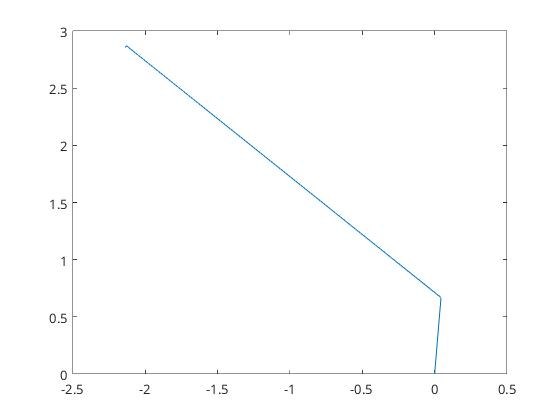
\includegraphics[angle=0,totalheight=50mm]{P1iigraph.jpg}
  \caption{Gradient Descent with Backtracking Line Search Solution Path}
  \label{fig:tabl}
\end{figure}

\section{Problem 2}

Using Newton's method gave me an optimal solution of $\mathbf{x} = \left( \begin{array}{cc} -2.1418\\2.8582 \end{array} \right)$ and an optimal value of -4.1423.

\begin{figure}[H] % "h" is where to place, h=here, t=top, b=bottom
  \centering
  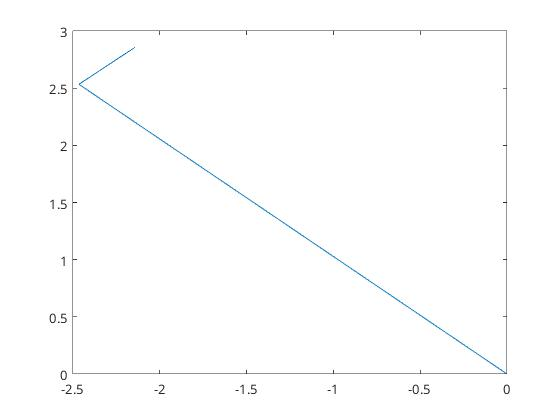
\includegraphics[angle=0,totalheight=50mm]{P2graph.jpg}
  \caption{Newton's Method Solution Path}
  \label{fig:tabl}
\end{figure}

\section{Problem 3}

Using both the gradient projection method and CVX gave me an optimal solution of $\mathbf{x} = \left( \begin{array}{cc} -.5183\\1.2500\\.6728 \end{array} \right)$ and an optimal value of -2.2524.

\end{document}
